\documentclass{article}

% --- load packages ---

\usepackage[margin=1in]{geometry} % change the margins
\usepackage{amsmath} % useful math environments and commands like align
\usepackage[colorlinks,bookmarks,bookmarksnumbered,allcolors=blue]{hyperref} % hyperlinks between references
\usepackage{graphicx}  % include images
\usepackage[caption=false]{subfig} % subfigures.  false option prevents conflicts in caption styling with other packages
\usepackage{booktabs} % better tables
\usepackage[capitalise]{cleveref} % better referencing. uses cref.
\usepackage[section]{placeins} % sometimes useful to prevent figures from floating out of a section
\usepackage{cite} % handles multiple citations in one command better
\usepackage{doi} % allow correct hypderlinking of DOIs
\usepackage{hyperref}


\begin{document}

\title{Homework 1}
\author{Jaron Ellingson}
% put in \date{} if you don't want a date to appear, or enter a specific date, otherwise default is today's date.
\maketitle

\section*{Abstract}

The following describes two optimization problems, one unconstrained and one constrained. The homework assignment explores using a optimization solver using python, specifically the \href{https://docs.scipy.org/doc/scipy/reference/generated/scipy.optimize.minimize.html}{scipy} library. It also explores topics such as dimensionality and accuracy trade-offs as well as convergence metrics.

\section{Brachistrochrone}

\subsection{Introduction}

The Brachistochrone problem seeks to minimize the time for a bead to travel between two points on a track by optimizing the track's position. Mathematically, it  

\begin{equation*}
\begin{aligned}
\text{minimizes} & \quad J=\sum_{i=1}^{n-1} \frac{\sqrt{\Delta x_i^2+\Delta y_i^2}}{\sqrt{H-y_{i+1}-\mu_{k}x_{i+1}} + \sqrt{H-y_i-\mu_i x_i} } \\
\text{with respect to} & \quad y_2 ... y_{n-1} \\
\text{and subject to} & \quad x_0=0, y_0=1, x_n=1, y_n=0,  \\
\end{aligned}
\end{equation*}

where $n$ is the number of control points (see \cref{fig:results}). Furthermore, $\mu$ is a friction coefficient, $H$ is the starting height of the bead, and $\Delta x = x_{i+1}-x_i$, $\Delta y = y_{i+1}-y_i$. For the complete problem formulation and parameters see the \href{https://byu.box.com/shared/static/iig80eoctek0lrs60avsmjxndc9sgk2m.pdf}{handout}.  I started with 4 control points and increased to 128, doubling the number of control points as I went. For this problem I choose to use scipy's ``BFGS" method.

\subsection{Results}

The result of the control points can be seen in \Cref{fig:results,fig:dimensionality}. The problem appears to find an relative optimum using 64 control points because the points do not move if you use more than 64 points. This can also be seen through \Cref{fig:dimensionality}, which shows four different metrics for how many control points are needed to solve this problem. The top subplot highlights that the difference between 64 and 128 control points does not give us much improvement in travel time. Additionally, the next two subplots show that 128 control points greatly increases the solve time and the function evaluations in a quadratic-like pattern. The final bottom subplot shows us that the number of iterations verses number of points appears linear. 


\begin{figure}[htbp]
	\centering
	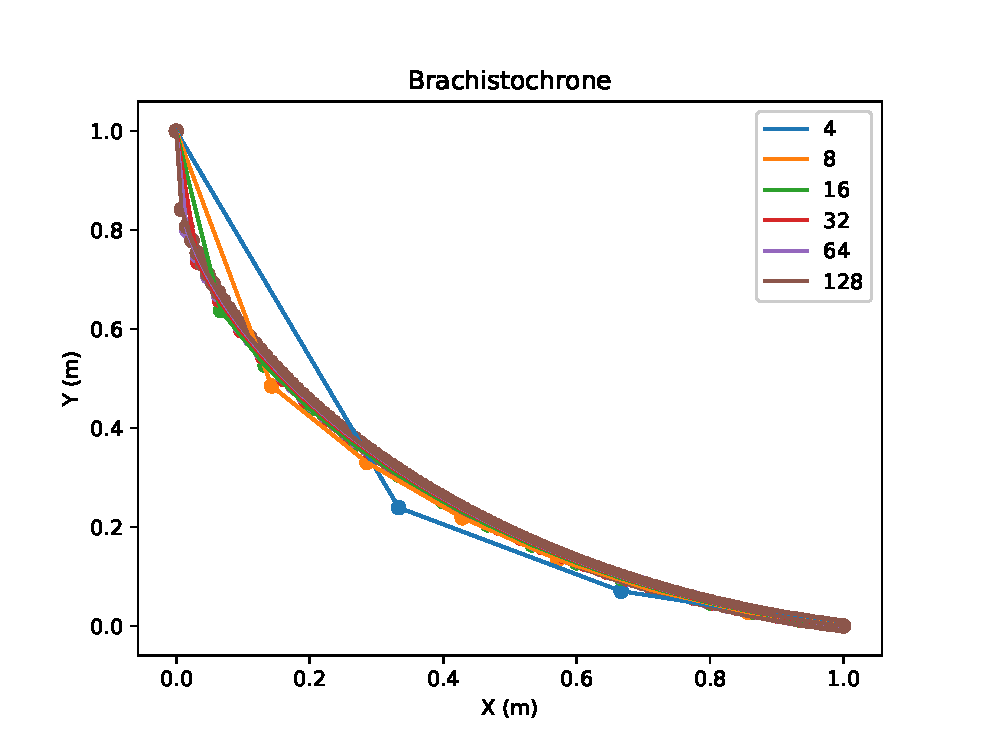
\includegraphics[width=0.75\textwidth]{figures/brachistrochrone.eps}
	\caption{Increasing the number of control points appears to converge onto a solution around 64 points.}
	\label{fig:results}
\end{figure}


These results make sense because I didn't provide the solver with a gradient function. This means that the solver had to take linear more directions to search in and at every iteration and had to evaluate the function n times to get the gradient. Therefore, function evaluations and solve time had $O(n^2)$ complexity and appear to be quadratic. 

Finally, while it appears to be bad to have higher dimensionality, especially with $O(n^2)$ complexity, 128 control points only took around 25 seconds to solve. If better accuracy is desired, then a higher number of control points and a longer solve time can be justified.




\begin{figure}[htbp]
	\centering
	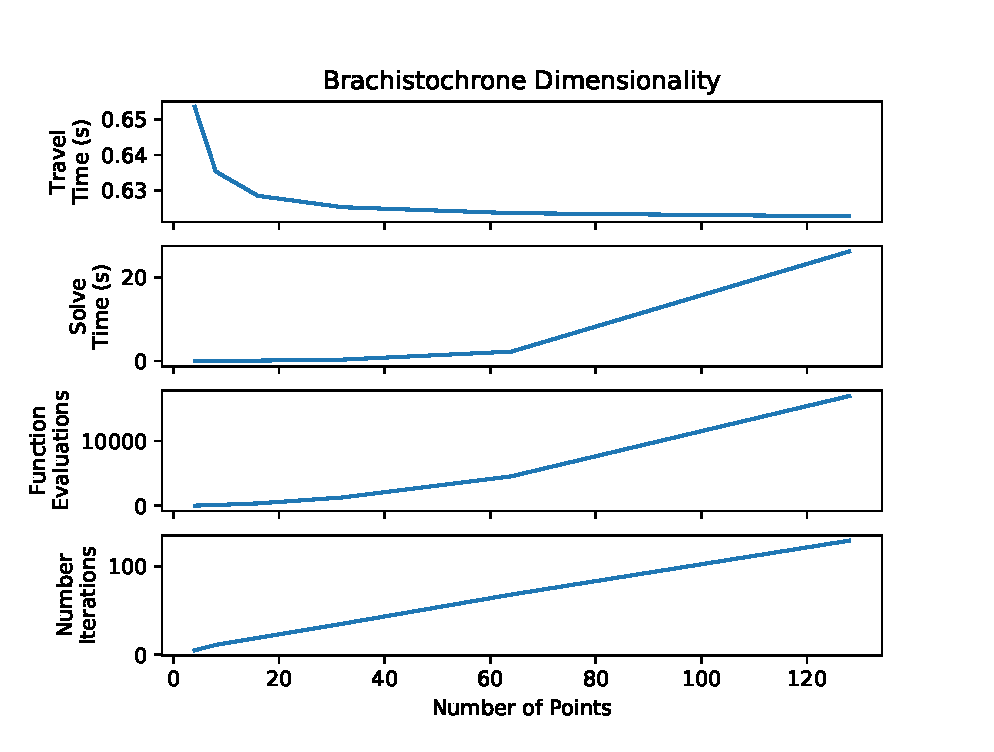
\includegraphics[width=0.75\textwidth]{figures/dimensionality.eps}
	\caption{The number of control points affects the final travel time, the time to solve the optimization, the number of function evaluations, and the number of iterations. Increasing the number of points appears to increase solve time and function quadratically and the number of iterations linearly.}
	\label{fig:dimensionality}
\end{figure}




\section{Truss}

\subsection{Introduction}

The next homework problem minimizes the mass of a 10-truss structure that holds a load suspended horizontally from a wall. The problem 

\begin{equation*}
\begin{aligned}
\text{minimizes} & \quad J= \sum_{i=1}^{n} Mass(A_i) \\
\text{with respect to} & \quad A_1 ... A_{n} \\
\text{subject to} & \quad A_i \ge 0.1 \quad \text{and} \quad | \sigma_i | \le \sigma_y \quad \forall i=1 ... n,
\end{aligned}
\end{equation*}

where $A_i$ is the cross-sectional area, $\sigma_i$ is the corresponding stress, and $\sigma_y$ is the yield stress. Once again, for further details please see the \href{https://byu.box.com/shared/static/iig80eoctek0lrs60avsmjxndc9sgk2m.pdf}{handout}. Notice that this problem requires constrained optimization. I used scipy's ``SLSQP" method that allows for these constraints to be added as arguments. I initialized each of the cross-sectional areas to be 0.1 m$^2$.


\subsection{Results}

The optimal truss mass of 1497.5 lbs took a total of 358 function calls. The results for each cross-sectional area and corresponding yield stress is shown in \Cref{tab:area_stress}. Notice that some of trusses remained at 0.1$m^2$ while other increased in size. It appears that the trusses that increased are more load bearing and are therefore more critical to the system.

\begin{table}[htb]
	\centering
	\caption{The final optimal result for each truss is shown with corresponding cross-sectional area and stress. Truss number 9 was allowed to have a max of 75e3 psi yield stress while all the others area allowed to have 25e3 psi yield stress.}
	\label{tab:area_stress}
	\begin{tabular}{c|c|c}
		\toprule
		Truss & Cross-Sectional Area (m$^2$)& Stress (psi) \\
		\midrule
		1 & 7.9 & 25e3 \\
		2 & 0.1 & 25e3 \\
		3 & 8.1 & -25e3 \\
		4 & 3.9 & -25e3 \\
		5 & 0.1 & 0 \\
		6 & 0.1 & 25e3 \\
		7 & 5.79827561 & 25e3 \\
		8 & 5.51543289 & -25e3\\
		9 & 3.67695526 & 37.5e3 \\
		10 & 0.14142136 & -25e3 \\
		\bottomrule
	\end{tabular}
\end{table}

I also included \Cref{fig:truss} to show the convergence of the optimizer. The first plot shows the mass of the system converging to 1497.5 lbs while the second shows the absolute max constraint violation converging to zero. This means that my initial estimate of 0.1m$^2$ violated the constraints but that overtime the constraints were satisfied and the program converged to a solution. 


\begin{figure}[htbp]
	\centering
	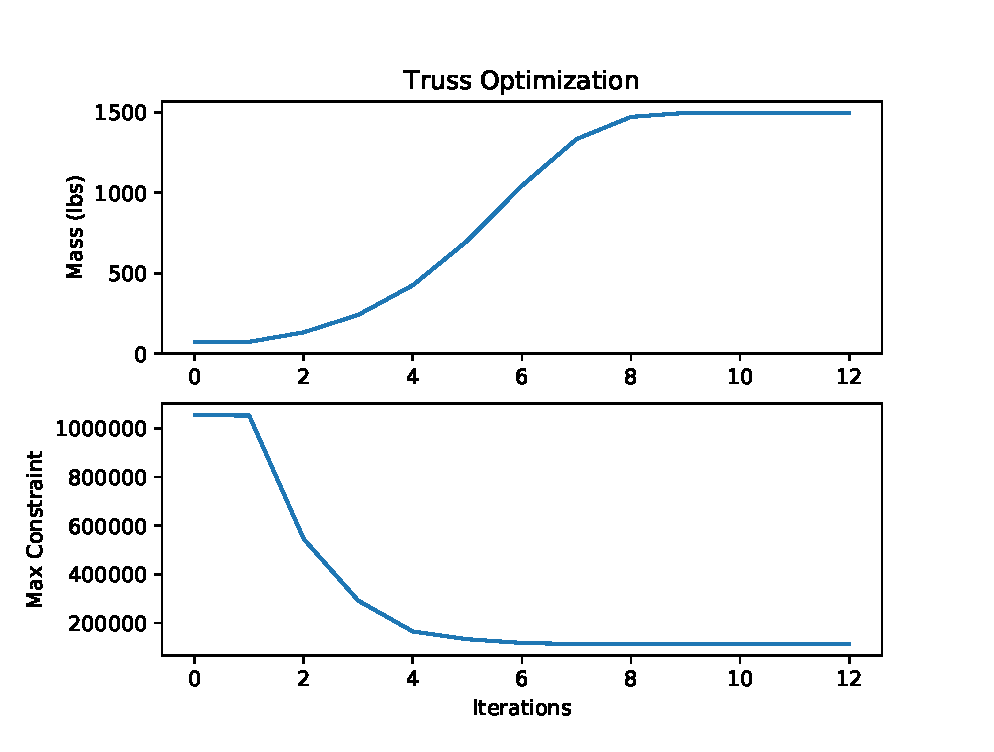
\includegraphics[width=0.75\textwidth]{figures/truss.eps}
	\caption{The convergence of the truss optimization is shown with mass and the max constraint violation on the y-axis verse the number of iterations on the x-axis.}
	\label{fig:truss}
\end{figure}




\section{Conclusions}

Both constrained and unconstrained non-linear optimization problems can be solved using the scipy library in python. The Brachistrochrone problem gives us insight in how increasing the number of control points affects the problem. The number of control points increases the solve time and number of functions evaluations with little improvement in the travel time. This trade off is important yet depends on the desired accuracy of the optimization.

The truss problem taught us more about what convergence of an optimization problem looks like. You can't only look at for a converging solution but also for the max constraint violations to converge to zero. The combination of these two convergences describe the convergence of the optimization.

% This is for the bibliography.  Note that it is using sample.bib 
% you would need to provide your own bibtex file.

%\bibliographystyle{unsrt}
%\bibliography{sample}


\begin{equation}
	Q=2\alpha\sigma^2\begin{bmatrix}
	\frac{dt^7}{252} & 0 & \frac{dt^6}{72} & 0 & \frac{dt^5}{30} & 0 & \frac{dt^4}{24} & 0\\
	0 & \frac{dt^7}{252} & 0 & \frac{dt^6}{72} & 0 & \frac{dt^5}{30} & 0 & \frac{dt^4}{24}\\
	\frac{dt^6}{72} & 0 & \frac{dt^5}{20} & 0 & \frac{dt^4}{8} & 0 & \frac{dt^3}{6} & 0 \\
	0 & \frac{dt^6}{72} & 0 & \frac{dt^5}{20} & 0 & \frac{dt^4}{8} & 0 & \frac{dt^3}{6} \\
	\frac{dt^5}{30} & 0 & \frac{dt^4}{8} & 0 & \frac{dt^3}{3} & 0 & \frac{dt^2}{2} & 0\\
	0 & \frac{dt^5}{30} & 0 & \frac{dt^4}{8} & 0 & \frac{dt^3}{3} & 0 & \frac{dt^2}{2} \\ 
	\frac{dt^4}{24} & 0 & \frac{dt^3}{6} & 0 & \frac{dt^2}{2} & 0 & \frac{dt^1}{1} & 0\\
	0 & \frac{dt^4}{24} & 0 & \frac{dt^3}{6} & 0 & \frac{dt^2}{2} & 0 & \frac{dt^1}{1}
	\end{bmatrix}.
\end{equation}

\end{document}